\newpage
\section{程序实现}
首先考虑输入的整数$n$,需要进行判断是否为纯数字并且为正整数。为此,我们考虑利用\verb|expr|操作来进行判断。
我们将$n$读入到\textbf{\$x}当中,并利用\verb|expr $x+0|判断是否为整数。如果返回值不为0,说明加法成功,即$n$为
整数。同时,为了不让错误信息输出到标准流当中,我们调用\verb|&>/dev/null|将错误信息丢弃。
\par 
接下来判断是否为负数。直接拿$n$与0进行比较大小即可,判断命令为 \verb|[ $x -le 0 ]|.
\par 
最后就是进行递归并且输出每次调用函数对应的\textbf{\$* \$1 \$2 $\cdots$},观察变化。对应的输出指令为\verb|echo $*|.
\par 
最终代码如下:

\lstset{language=bash}
\begin{lstlisting}[caption = code]
    #!/bin/sh
    work(){
        echo $*
        if [ $1 = 0 ]
        then 
            echo "$2 -> $4"
        else
            x=$(expr $1 - 1)
            work $x $2 $4 $3
            echo "$2 -> $4"
            work $x $3 $2 $4  
        fi
    }   
    while true
    do
        echo "Please input the number of disks:"
        read x
        expr $x + 0 &>/dev/null
        if [ $? = 0 ] 
        then
            if [ $x -le 0 ] 
            then echo "Please input a correct number!"
            else
                work $x 1 2 3
                exit 0
            fi
        else
            echo "Please input a correct number!"
        fi
    done  
    exit 0
\end{lstlisting}
\par 
并且得到以下输出:
\begin{figure}[h]
    \centering
    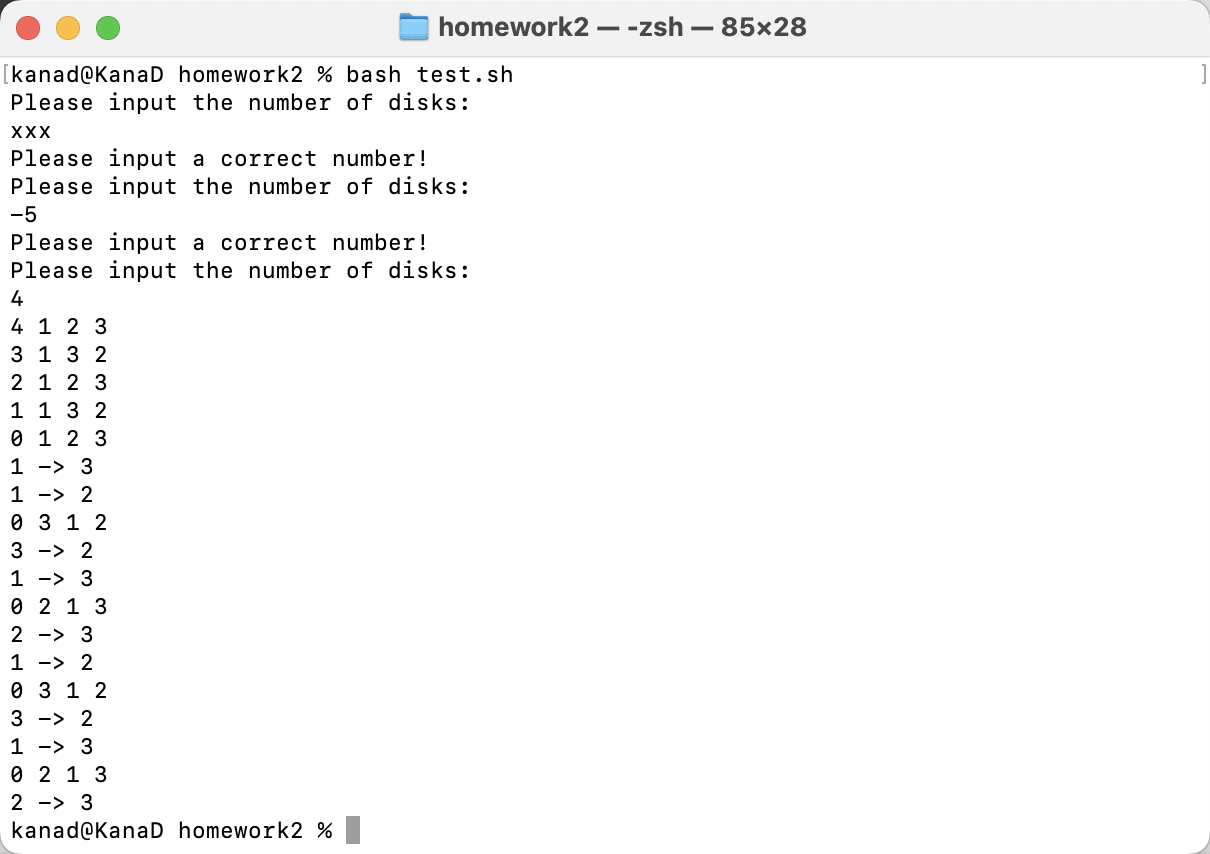
\includegraphics[width=12cm]{./result.png} 
    \caption{result} 
\end{figure}
\par 
由此可见,在递归的情况下,\textbf{\$* \$1 \$2 $\cdots$}的值也会递归变化并逐级变回来。